\documentclass[12pt, a4paper]{report}
\usepackage[italian]{babel}
\usepackage[T1]{fontenc}
\usepackage[sfdefault]{noto}
\usepackage{graphicx}
\usepackage{multirow}
\usepackage{enumitem}
\usepackage{hyperref}
\hypersetup{pdfborder = 0 0 0 }
\usepackage{wrapfig}
\usepackage{color}
\linespread{1.3}
\textwidth=450pt\oddsidemargin=0pt
\begin{document}
\begin{titlepage}
\vspace{15mm}
\begin{center}
  
\includegraphics{Images/uniboLogo}
\end{center}
\begin{center}
{\normalsize{\bf Corso di Laurea Magistrale in Informatica}}\\
\vspace{5mm}
{\normalsize{\bf Anno Accademico 2018/2019}}\\
\vspace{20mm}
{\Large{\bf Software Architecture}}\\
\vspace{10mm}
{\Huge{\bf Kubernetes}}\\
\vspace{25mm}
\end{center}
\begin{flushright}
{\large{Matteo Marchesini\\0000856336\\matteo.marchesini12@studio.unibo.it}}
\end{flushright}
\end{titlepage}
\tableofcontents
\chapter{Descrizione del sistema}
\begin{center}
  
\includegraphics[scale = 0.9]{Images/kubernetesLogo}
\end{center}
Kubernetes è un sistema open source per la gestione di applicazioni containerizzate tra più host; fornisce un meccanismo per il deployment, la manutenzione e lo scaling di applicazioni. È stato inizialmente sviluppato dal team di Google, per poi passare nel 2015 sotto il controllo del \textit{Cloud Native Computing Foundation (CNCF)}, che attualmente lo supporta.\\ Al giorno d'oggi è uno dei sistemi di orchestrazione per applicazioni conteinerizzate più utilizzato in assoluto, con una vastità di utenti, partners e una comunità di development attiva. Non a caso tre dei quattro maggior providers di servizi Cloud - Microsoft, IBM e Google - offrono piattaforme di Container as a Service (CaaS) basate su Kubernetes. I servizi che Kubernetes mette a disposizione sono molteplici: fornisce un ambiente la gestione di container, microservizi e piattaforme cloud. Inoltre organizza l'infrastruttura di rete e di archiviazione per conto dell'utente.\\
In generale un sistema distribuito necessita di più componenti per il corretto funzionamento, alcune open source e altre commerciali; invece Kubernetes da solo fornisce uno scenario in cui le componenti lavorano insieme, andando così a formare un unico componente combinando la semplicità del Platform as a Service (PaaS) con la flessibilità dell'Infrastructure as a Service (IaaS).\\
L'orchestrazione di container ha avuto un profondo impatto in ogni aspetto del software development e deployment moderno; in particolare ha influenzato l'architettura del Platform as a Service, fornendo un aperto ed efficiente modello per il packaging, deployment, isolamento, scaling e rolling upgrade. Kubernetes svolgerà un ruolo cruciale nell'utilizzo di container da parte di imprese e start-up emergenti.
\\L'oggetto di questo report è di studiare tutto ciò che riguarda e circonda l'architettura di Kubernetes.
\chapter{Contesto}
\section{Scopo del sistema}
In questo capitolo verrà discusso lo scopo di Kubernetes e la sua interazione con le entità esterne, nonchè i principali casi d'uso. \\
Kubernetes, come introdotto nel Capitolo 1, è un sistema di orchestrazione di container e per questo motivo si occupa principalmente di \textbf{deployment}, \textbf{scaling} e \textbf{management} di applicazioni containerizzate. Di seguito viene definito ognuno di questi tasks:
\begin{itemize}
\item \textbf{Deployment}: gestisce la distribuzione di applicazioni assegnando ai nodi del cluster ciascuna istanza dell'applicazione. Il deployment in Kubernetes può essere eseguito in una varietà di ambienti con pattern differenti, ed esistono appunto diversi modelli, quali:
\begin{itemize}
  \item Container as a Service (CaaS);
  \item Public Cloud - Infrastructure as a Service (IaaS);
  \item Utilizzo on-premises all'interno di data center;
  \item Deployment ibrido
\end{itemize}
\item \textbf{Scaling}: permette di ridimensionare l'applicazione a seconda delle esigenze dell'utente, andando a modificare le dimensioni del cluster e il numero di repliche dei pod. Un \textbf{pod} è il più piccolo oggetto deployabile nel modello a oggetti di Kubernetes e può incapsulare un singolo container o più container che necessitano di lavorare insieme.
\item \textbf{Management}: fornisce un'interfaccia per la gestione dei cluster e delle applicazioni containerizzate. Un cluster di Kubernetes viene ospitato e gestito da un venditore commerciale, quali ad esempio Google Container Engine (GKE), Amazon EC2 Container Service e Azure Container Service di Microsoft, che offrono servizi di CaaS nel cloud pubblico. Molti utenti hanno iniziato ad usare Kubernetes attraverso Google Container Engine, essendo uno dei primi servizi di gestione di Kubernetes nel mercato.
\end{itemize}
\section{Entità esterne}
Nella figura seguente è espresso il \textit{system context diagram} di Kubernetes, che definisce le relazioni tra esso e le entità esterne.
\begin{center}
  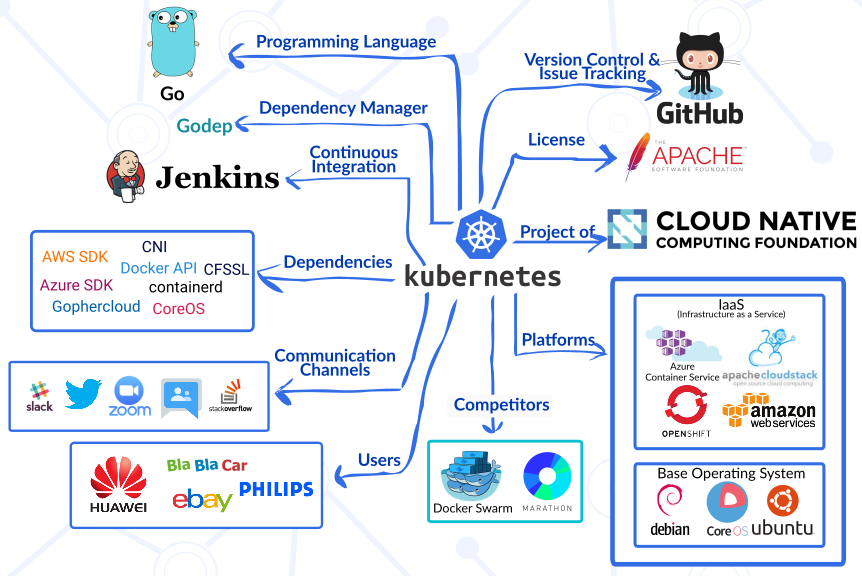
\includegraphics[scale = 0.6]{Images/ContextModelDiagram}
\end{center}
Le entità di maggior rilievo all'interno del diagramma e che verranno analizzate in seguito sono gli stakeholders, il development, le piattaforme e i concorrenti.
\subsection{Stakeholders}
Per poter comprendere al meglio il concetto di stakeholder all'interno di un progetto così grande come quello di Kubernetes, è necessario introdurre il \textbf{Cloud Native Computing Foundation} (CNCF).\\
CNCF è nato 
\subsection{Development}
\subsection{Piattaforme}
\subsection{Concorrenti}
\chapter{Drivers architetturali}
\chapter{Struttura}
\chapter{Funzioni}
\chapter{Comportamento}
\chapter{Razionale}
\chapter{Aspetti analitici}
\chapter{Stili architetturali simili o derivati}
\chapter{Referenze}
\end{document}
